\begin{figure*}[!tp]
\centering
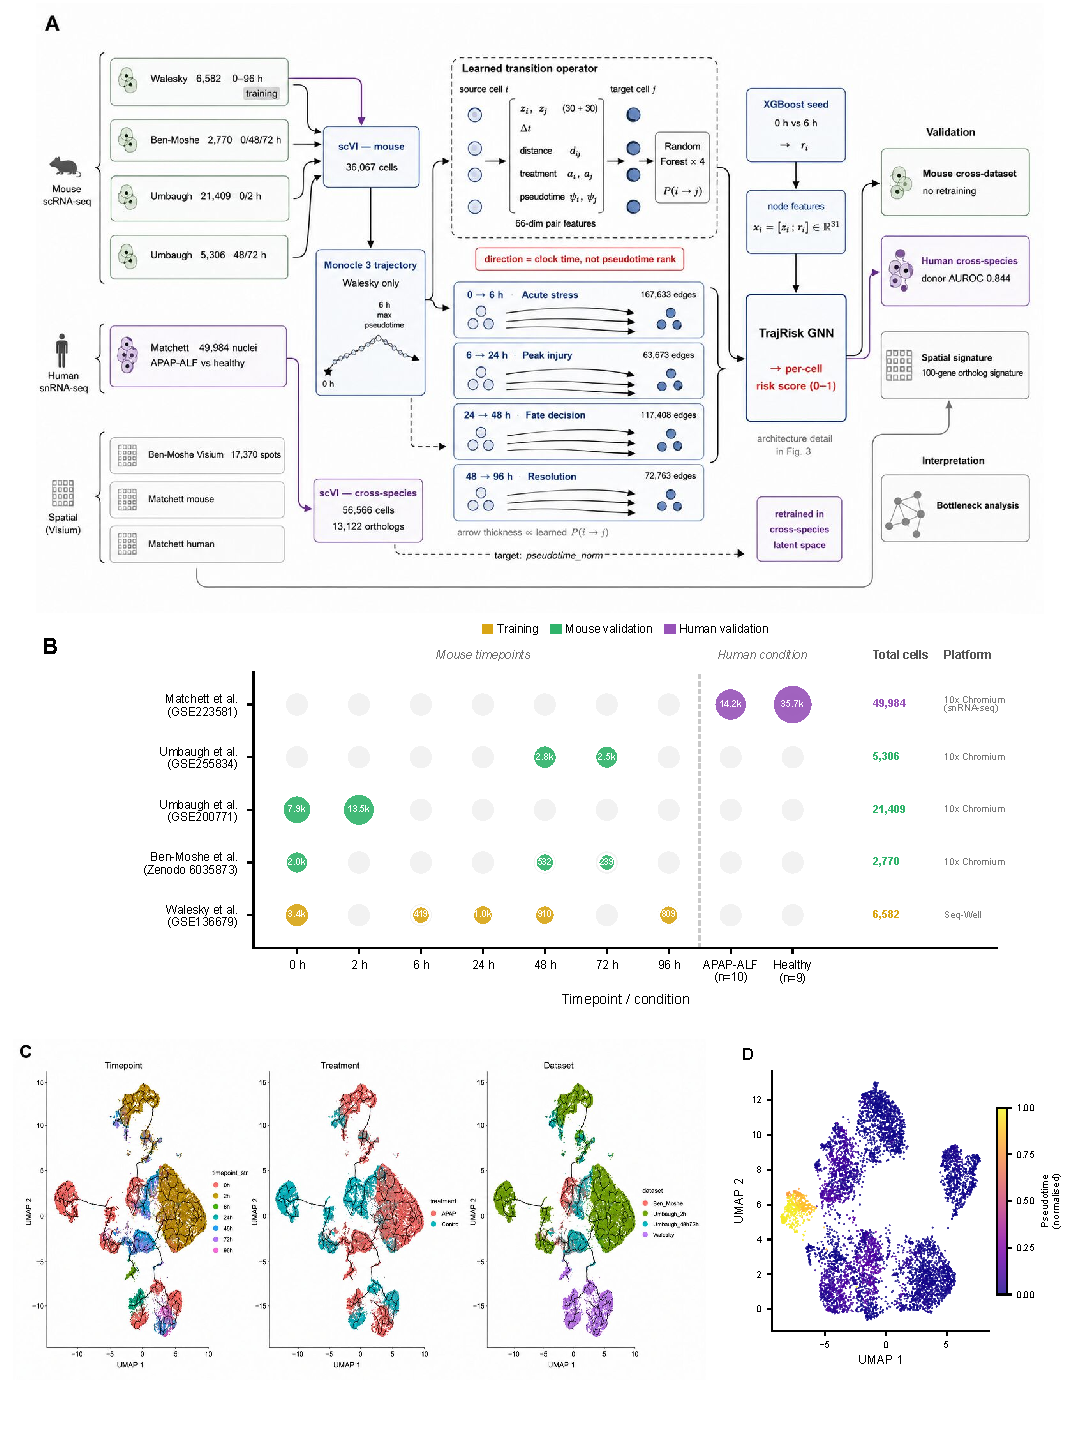
\includegraphics[width=\textwidth,trim={0.000bp 395.000bp 0.000bp 0.000bp},clip]{figures/figure_1.pdf}
\caption{\textbf{\FigOneTitle{}} \textbf{(A)} \FigOneA{}}
\label{fig:1}
\end{figure*}
\begin{figure*}[!tp]
\centering
\ContinuedFloat
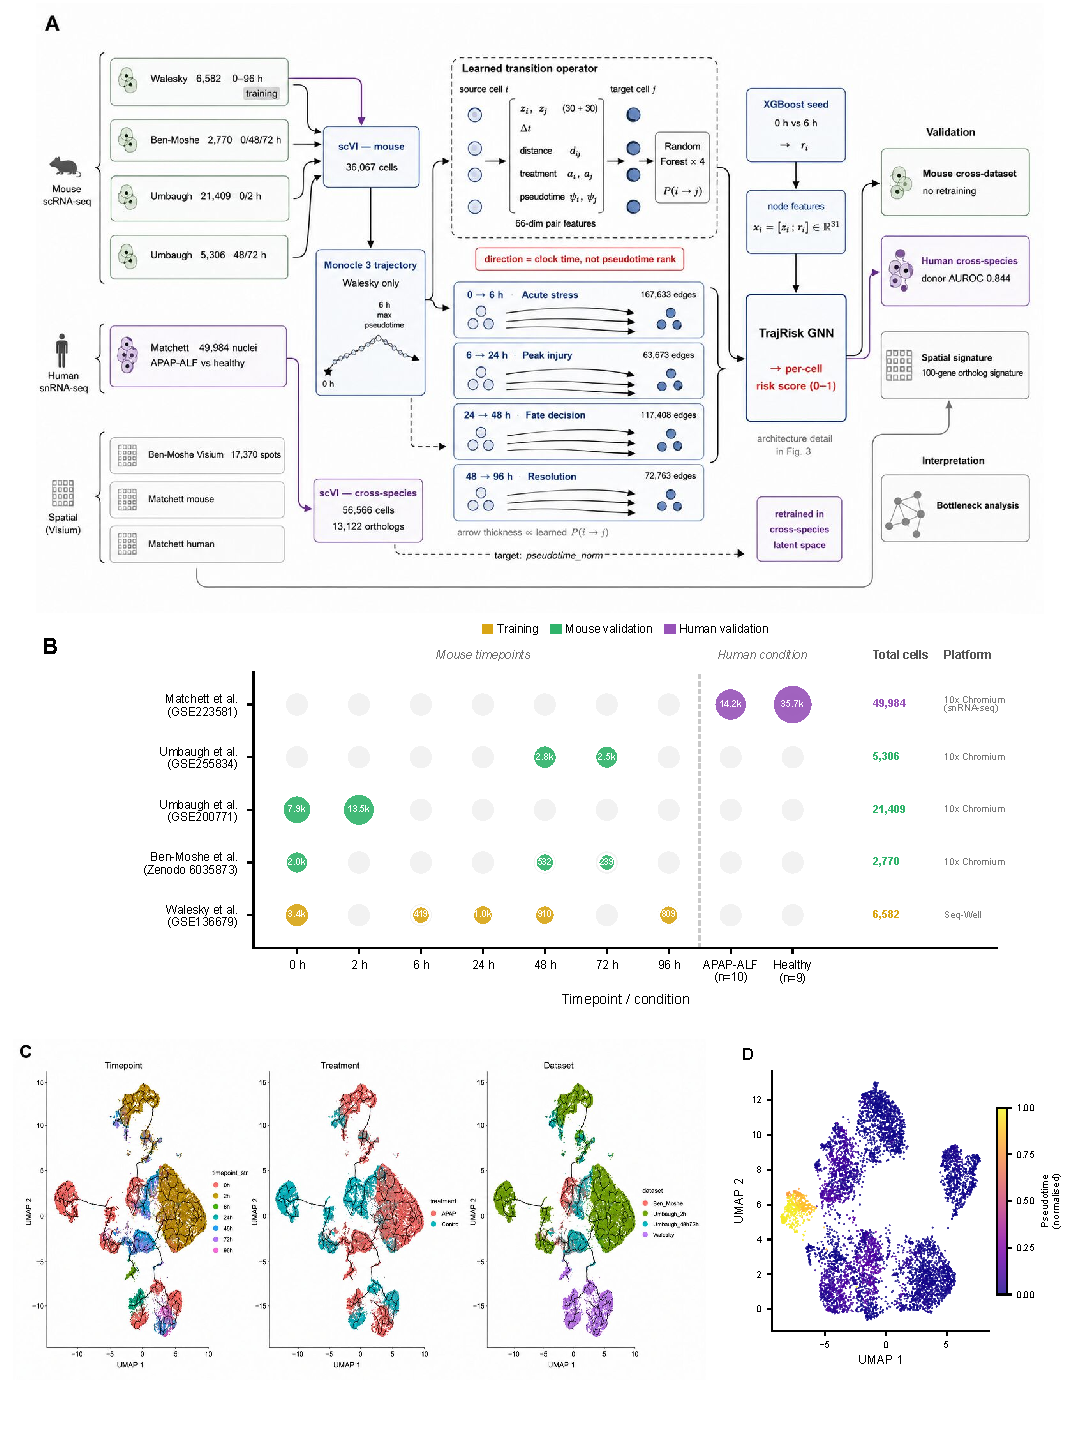
\includegraphics[width=\textwidth,trim={0.000bp 192.000bp 0.000bp 299.000bp},clip]{figures/figure_1.pdf}
\par\vspace{8pt}
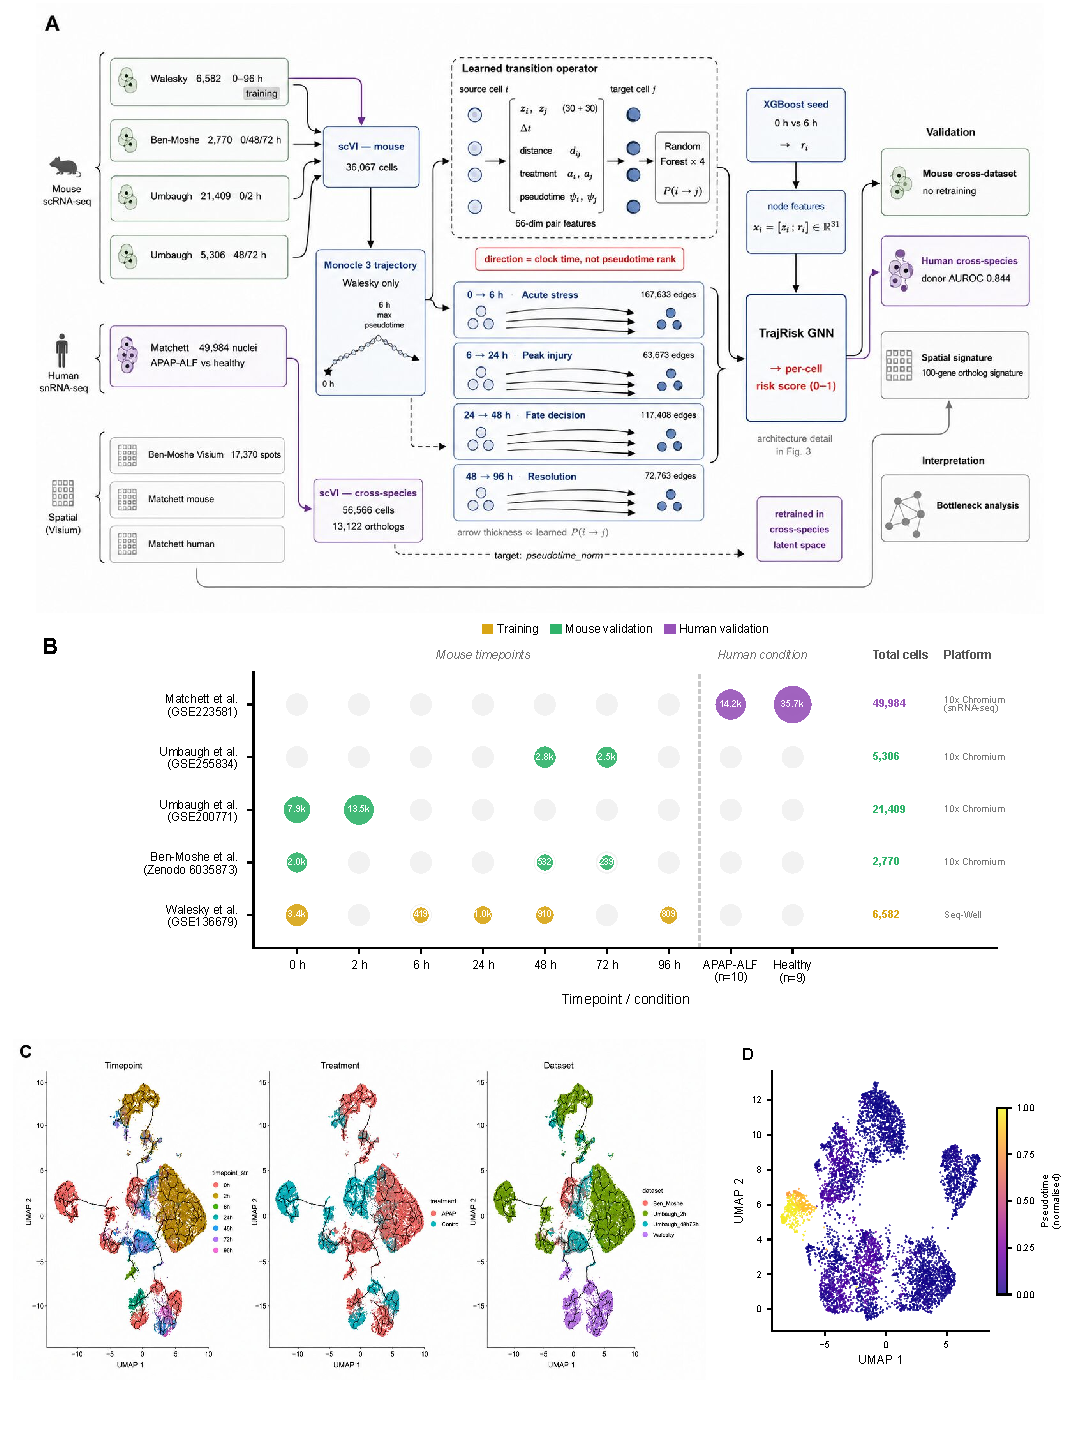
\includegraphics[width=\textwidth,trim={0.000bp 4.000bp 0.000bp 502.000bp},clip]{figures/figure_1.pdf}
\caption{\textbf{\FigOneTitle{} (continued)} \textbf{(B)} \FigOneB{} \textbf{(C)} \FigOneC{} \textbf{(D)} \FigOneD{} \FigOneNotes{}}
\end{figure*}
